\subsection{Computation of derivatives} \label{sec:derivatives}

Computation of derivative quantities such as gradient and Laplacian is important in data analysis.
Since simulation data can rarely be captured by closed-form formulae, we use finite differences. In
this section, we use 32 bits (instead of 16) for quantization to ensure enough precision for finite
differences. We always perform finite differences on the finest (original) resolution. This decision
avoids the problem of computing distances between quantities defined on grids of different sizes,
because we are unaware of any widely accepted solutions to this problem.~\Cref{sec:gradient}
discusses gradient computation, and~\Cref{sec:laplacian} discusses computation of the Laplacian.

\subsubsection{Gradient computation} \label{sec:gradient}

\begin{figure*}[t]
\centering
\subcaptionbox{\emph{boiler}}{%
{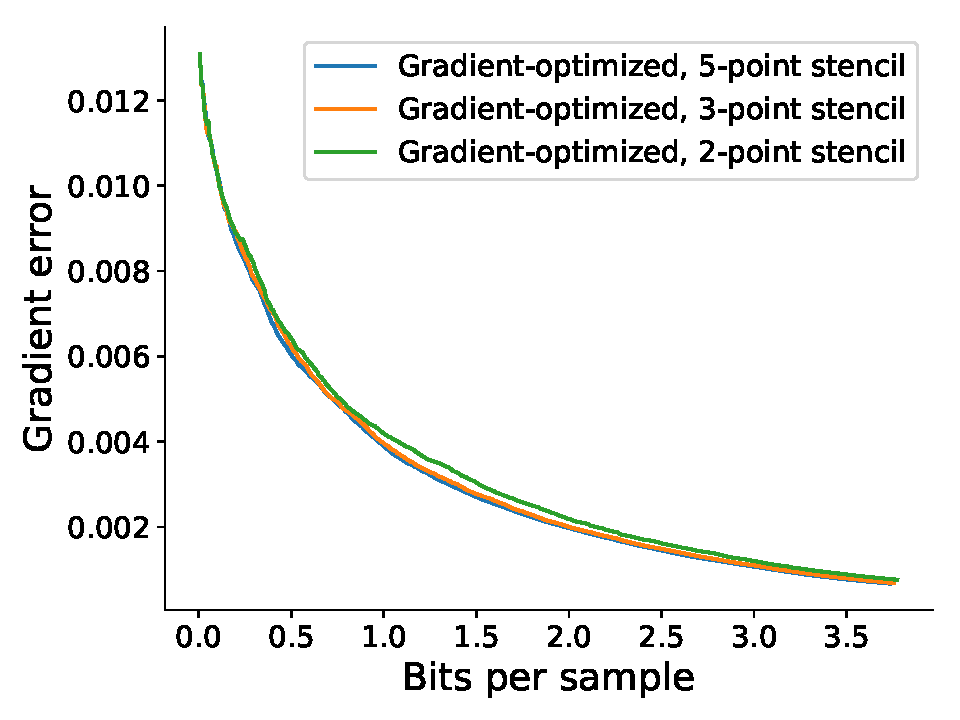
\includegraphics[width=0.24\linewidth]{gradient/gradient-optimized-boiler}}}
\subcaptionbox{\emph{diffusivity}}{%
{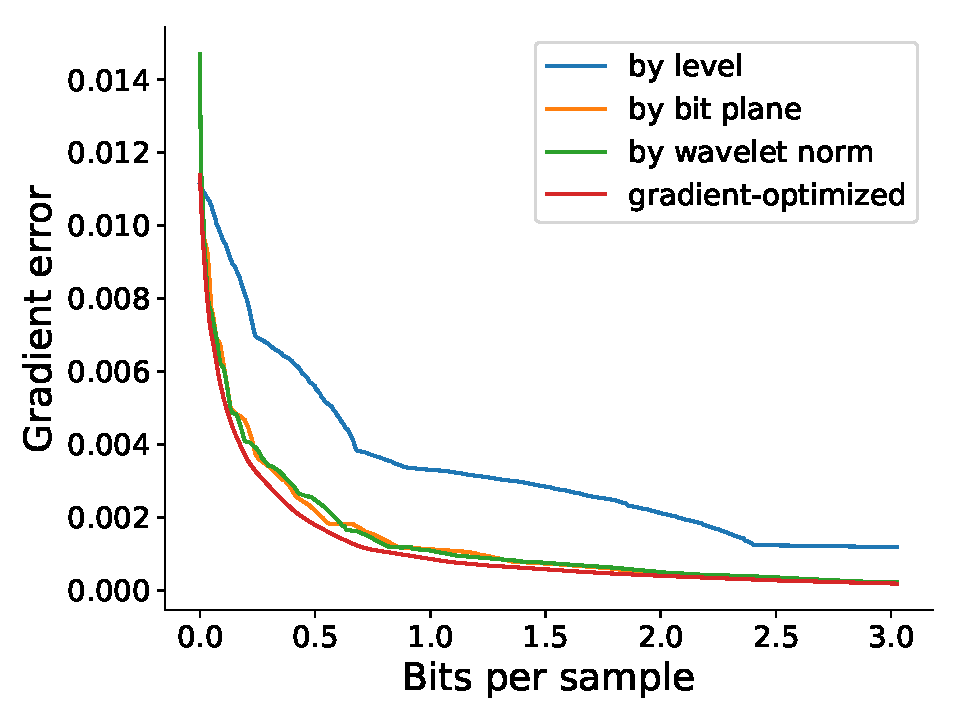
\includegraphics[width=0.24\linewidth]{gradient/gradient-optimized-diffusivity}}}
\subcaptionbox{\emph{turbulence}}{%
{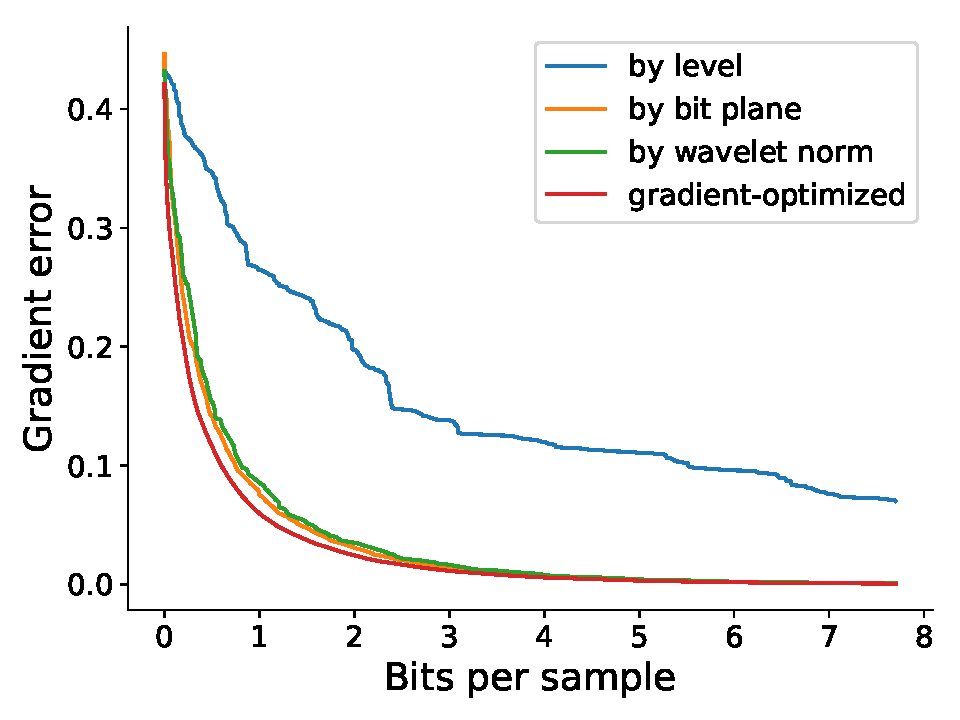
\includegraphics[width=0.24\linewidth]{gradient/gradient-optimized-turbulence}}}
\subcaptionbox{\emph{pressure}}{%
{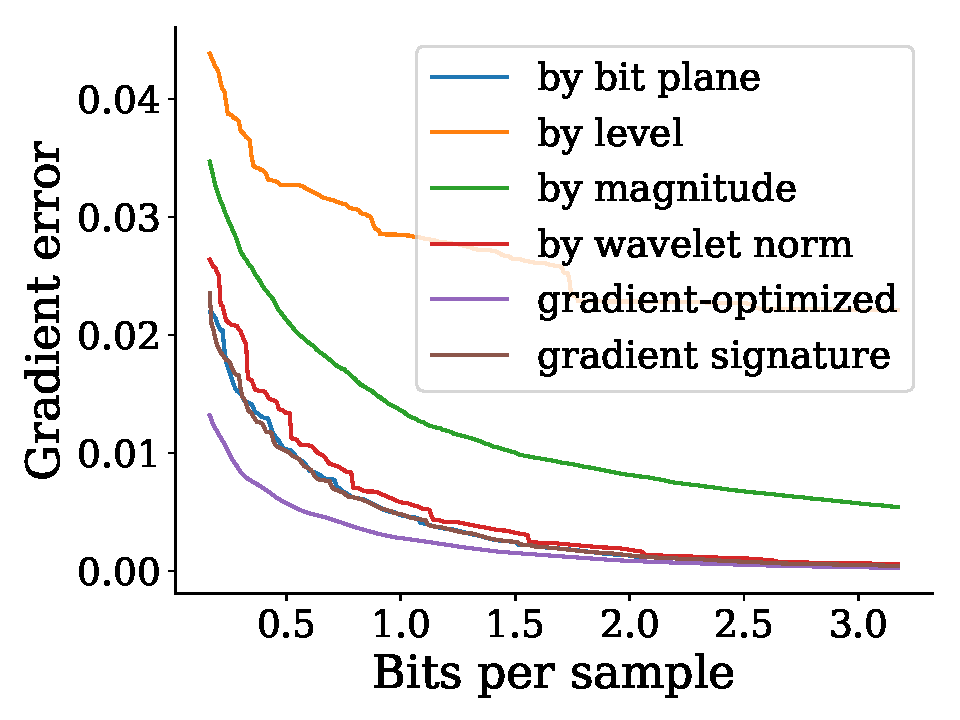
\includegraphics[width=0.24\linewidth]{gradient/gradient-optimized-pressure}}}
\caption{Gradient error of reconstructed functions. Lower gradient error is better. Leading zero
packets are removed, and the plots are truncated in the same way as in~\Cref{fig:rmse-optimized}.
The trend in error, in all cases, is $\sgop < \sgsg \approx \sbit < \swav < \smag < \slvl$.}
\label{fig:gradient-error-comparison}
%\vspace{1em}

\centering
\subcaptionbox{\emph{by level} (\slvl)}{%
{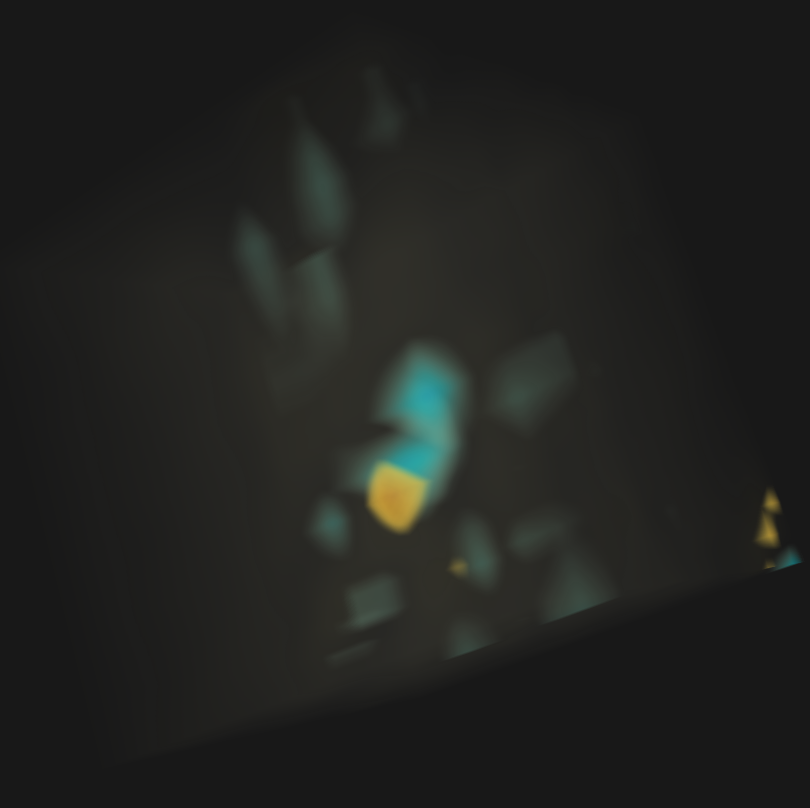
\includegraphics[width=0.16\linewidth]{gradient/gradient-turbulence-level}}}
\subcaptionbox{\emph{by bit plane} (\sbit)}{%
{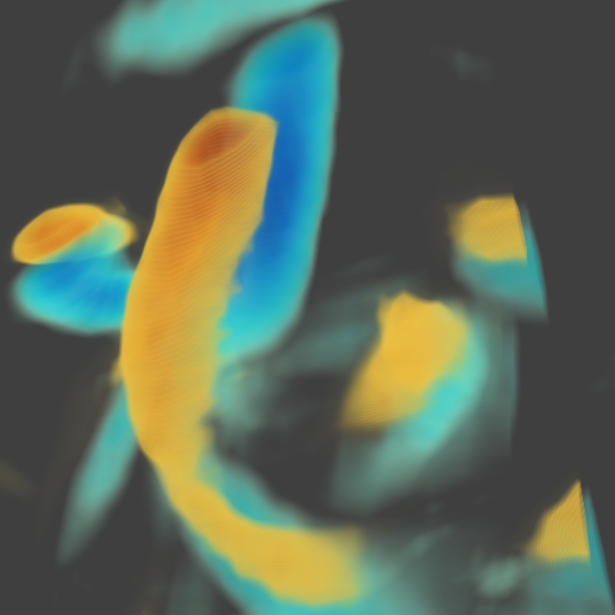
\includegraphics[width=0.16\linewidth]{gradient/gradient-turbulence-bit-plane}}}
\subcaptionbox{\emph{by wavelet norm} (\swav)}{%
{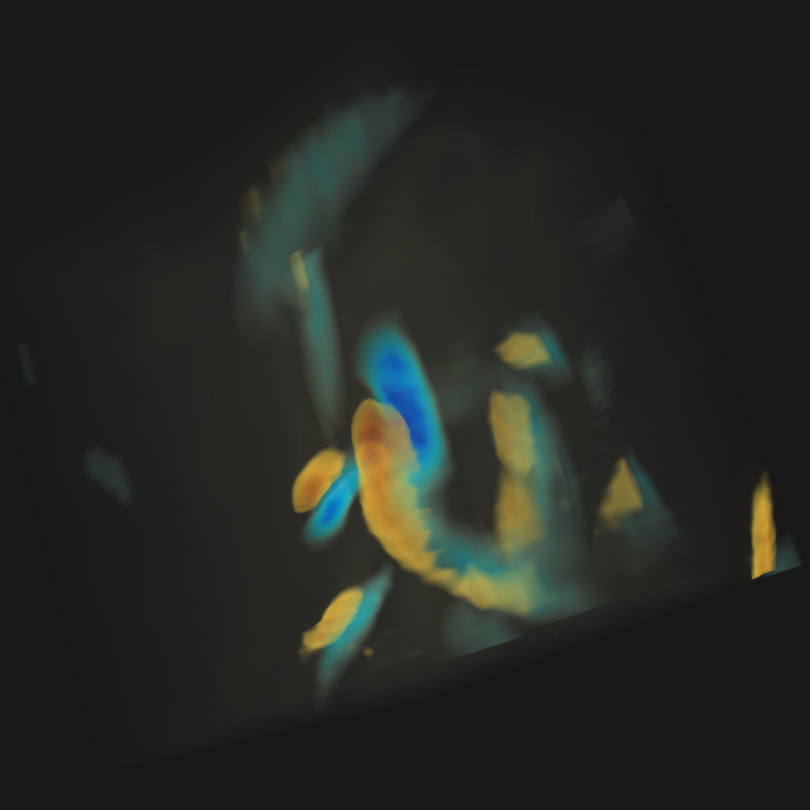
\includegraphics[width=0.16\linewidth]{gradient/gradient-turbulence-wavelet-norm}}}
\subcaptionbox{\emph{by magnitude} (\smag)}{%
{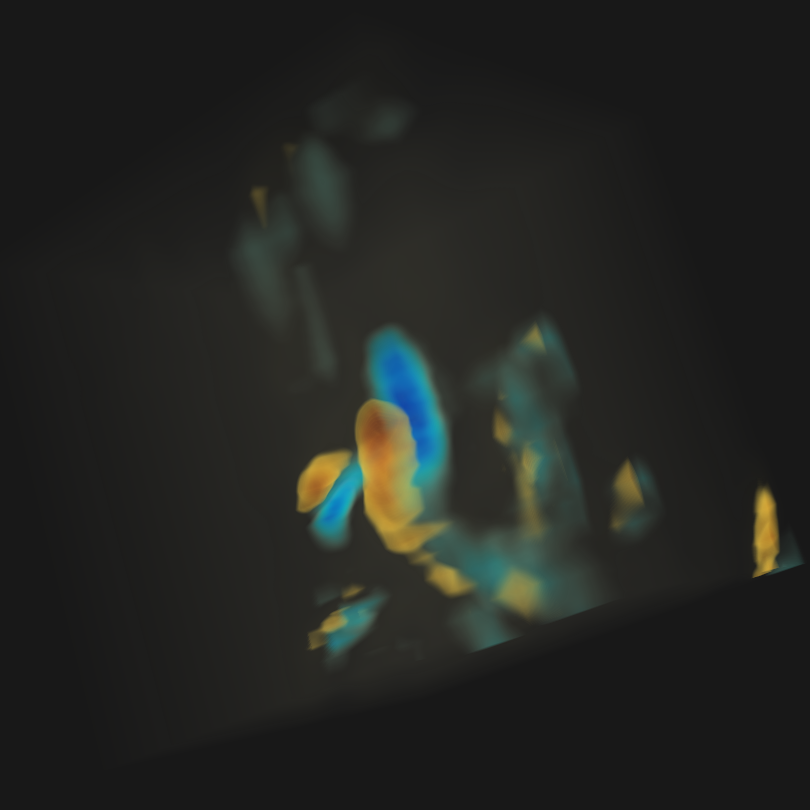
\includegraphics[width=0.16\linewidth]{gradient/gradient-turbulence-magnitude}}}
\subcaptionbox{\emph{by signature} (\sgsg)}{%
{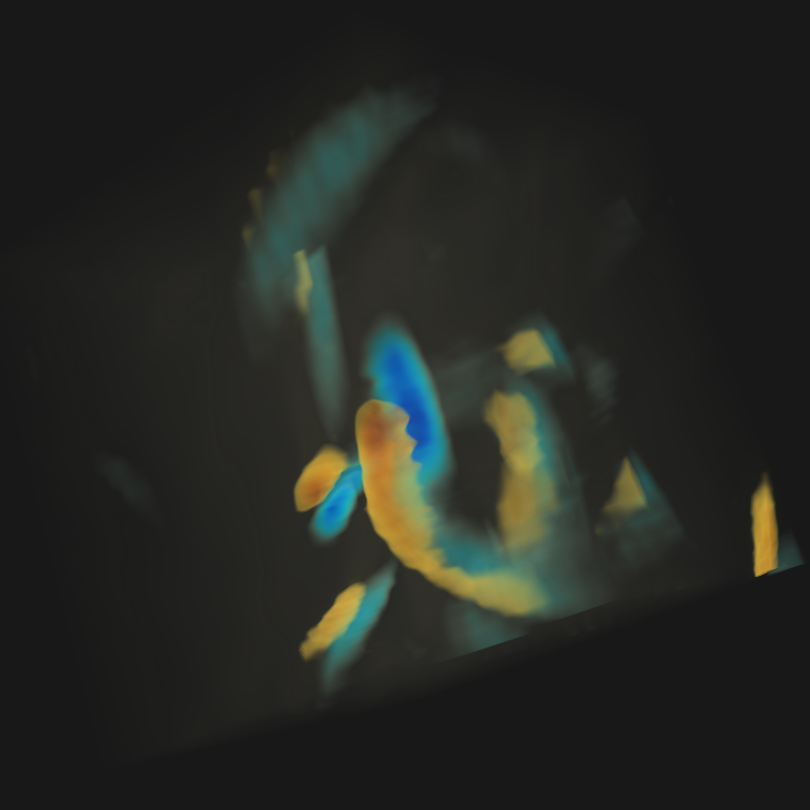
\includegraphics[width=0.16\linewidth]{gradient/gradient-turbulence-signature.png}}}
\subcaptionbox{\emph{ground truth}}{%
{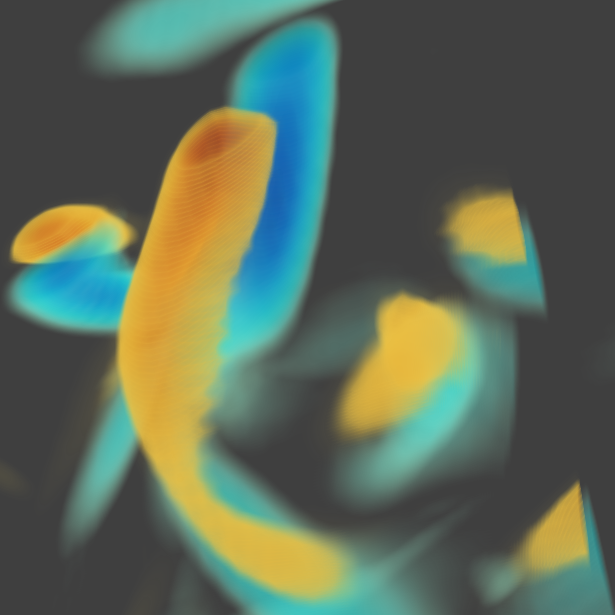
\includegraphics[width=0.16\linewidth]{gradient/gradient-turbulence-groundtruth.png}}}
\caption{$x$-component of the ($64^3$) gradient field of \emph{turbulence}, reconstructed at 0.2
bps. The gradient field produced by \sbit is more accurate than one produced by either \swav or
\sgsg (compare orange features).}
\label{fig:gradient-rendering-diff}
\end{figure*}

\begin{figure}[h]
\centering
\subcaptionbox{\emph{by bit plane} (\sbit)}{%
{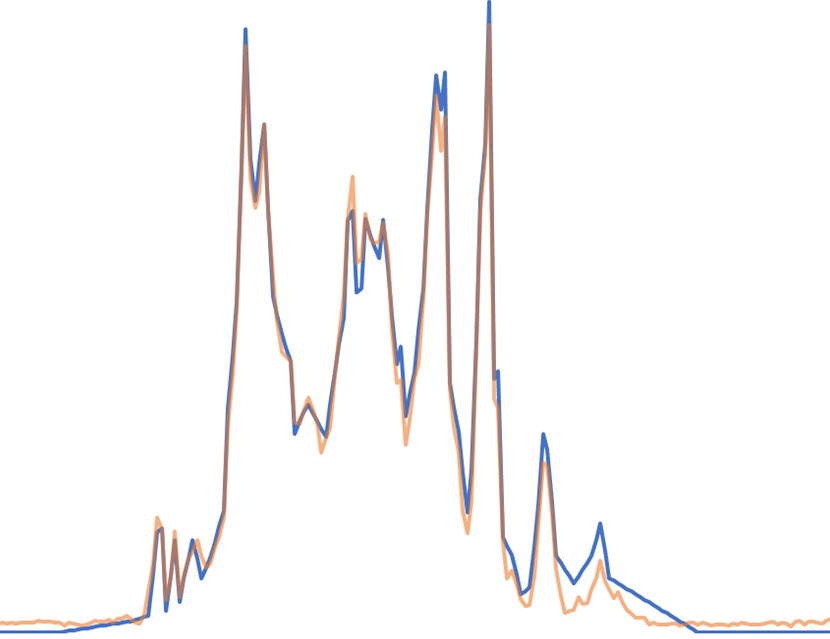
\includegraphics[width=0.48\linewidth]{gradient/gradient-bit-plane}}}
\subcaptionbox{\emph{by wavelet norm} (\swav)}{%
{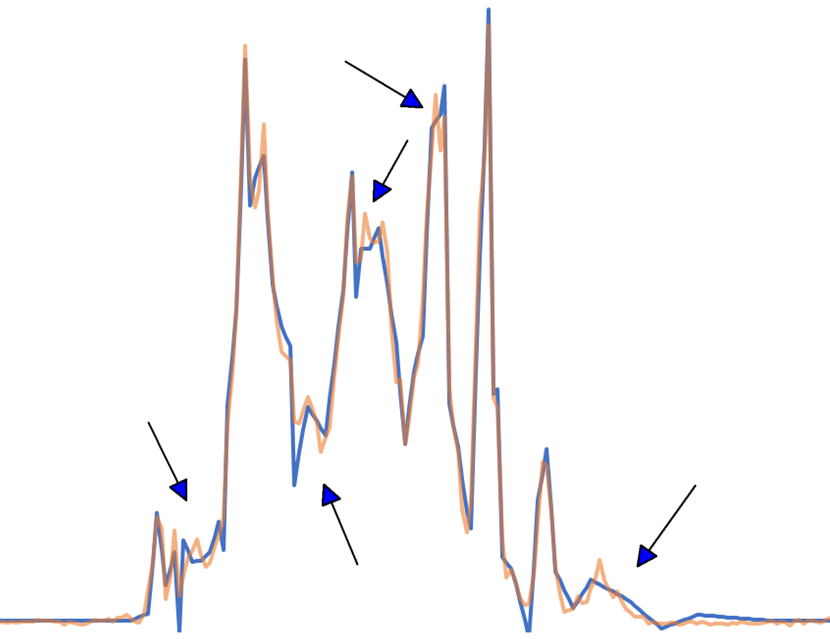
\includegraphics[width=0.48\linewidth]{gradient/gradient-wavelet-norm}}}
\caption{A 1D line extracted from \emph{plasma}, and reconstructed using \sbit and \swav at 0.6 bps.
The original data is in orange and the reconstructions are in blue. \swav captures well the function
values in low-gradient regions, where \sbit struggles (red arrows). However, \sbit retains the shape
of the original function well in areas of both low and high gradients, where \swav instead produces
smooth approximations (blue arrows). \sbit therefore is better for derivative computations, where a
function's shape (or its relative values) matters more than its absolute values.}
\label{fig:bit-plane-vs-wavelet-norm-gradient}
\end{figure}

The gradient of a given function 3D $f$ at a grid point \mbox{$\x = (x,y,z)$} is the vector
$(\frac{\partial f}{\partial x},\frac{\partial f}{\partial y}, \frac{\partial f}{\partial y})$. We
compute the derivative in each dimension using a five-point stencil, i.e., \mbox{$\frac{\partial
f}{\partial x} \approx \frac{1}{12}f(x-2,y,z) - \frac{2}{3}f(x-1,y,z) + \frac{2}{3}f(x+1,y,z) -
\frac{1}{12}f(x+2,y,z)$.} 
Using~\Cref{alg:greedy}, we compute a \emph{gradient-optimized} stream, \sgop, that minimizes the
difference between the reconstructed gradient field and the original gradient field. The error at
each grid point $\x_i$ is the squared L\textsubscript{2} norm of the difference between two gradient
vectors, i.e., $\norm{\nabla \tilde{f}(\x_i) - \nabla f(\x_i)}^2$, where $\tilde{f}$ is an
approximation of $f$ at low bit rates. The overall error, defined over the whole field, is
$\err(\nabla \tilde{f}, \nabla f) = \sqrt{\frac{1}{n} \sum_{i=1}^{n}{\norm{\nabla
\tilde{f}(\x_i)-\nabla f(\x_i)}^2}}$.

\Cref{fig:gradient-error-comparison} shows the gradient error incurred by different streams for four
data sets. In general, we observe the ordering of performance (from best to worst) as: \sgop, \sgsg,
\sbit, \swav, \smag, \slvl. This ordering can also be seen in~\Cref{fig:gradient-rendering-diff},
where the $x$-component of the gradient field for \emph{tuburlence} is reconstructed and rendered,
at 0.2 bps. Unlike the RMSE case, \sbit produces better approximations of the gradient field,
compared to \swav.

To further investigate this behavior, a 1D line is extracted from \emph{plasma}, and reconstructed
using \sbit and \swav at 0.6 bps (see~\Cref{fig:bit-plane-vs-wavelet-norm-gradient}). Because the
coarse-scale coefficients in \sbit are not accurate enough, the reconstruction from \sbit is
inaccurate in areas of low gradients. In contrast, the \swav's reconstruction is accurate in
low-gradient areas, but lacks the resolution to resolve the high-gradient areas, because \swav
frequently intersperses bits that improve resolution and bits that improve precision, unlike \sbit,
which always streams bits that improve resolution first. Therefore, \swav tends to produce a
``smoother'' reconstruction that \emph{on average} (i.e., in terms of RMSE) is close to the original
function. \sbit, on the other hand, tends to capture well the function's shape (due to fine-scale
bits), but the whole function can be ``shifted'' slightly due to the lack of precision in
coarse-scale coefficients. However, the error caused by this shifting reduces significantly when
taking gradient, which cancels any constant shift. \sbit, therefore, works better than \swav for
gradient computation, because it is better able to retain sharp features.

\duong{talk about the by-level, by-magnitude, and signature}
\duong{explain the ``bumpiness'' in the by wavelet norm}

\subsubsection{Laplacian computation}\label{sec:laplacian}

\begin{figure*}[h]
\centering
\subcaptionbox{\emph{boiler}}
{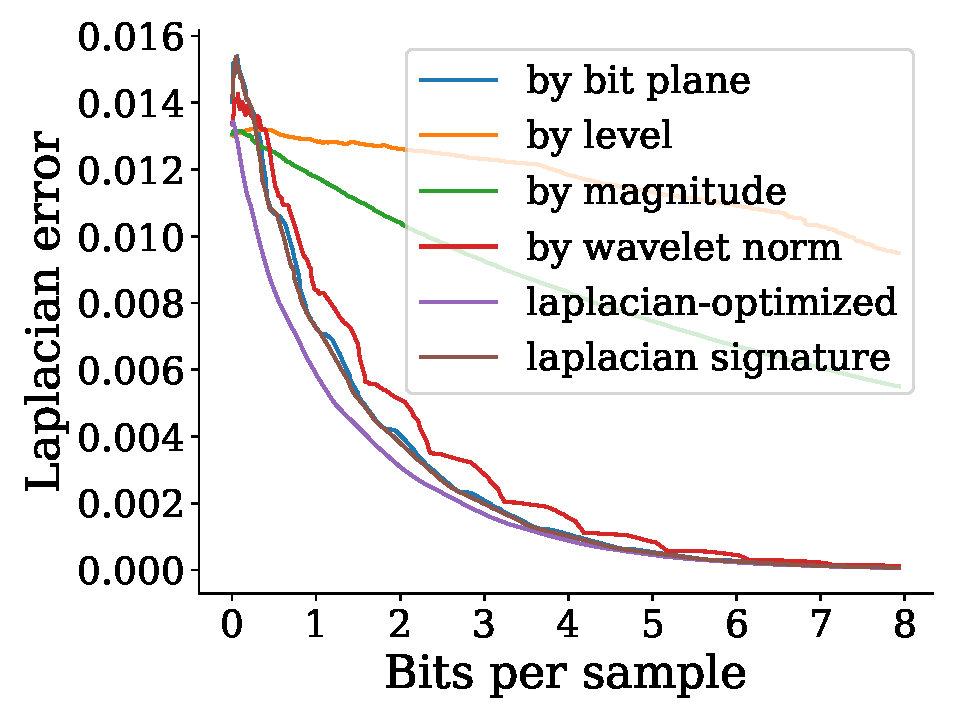
\includegraphics[width=0.24\linewidth]{laplacian/laplacian-optimized-boiler}}
\subcaptionbox{\emph{diffusivity}}
{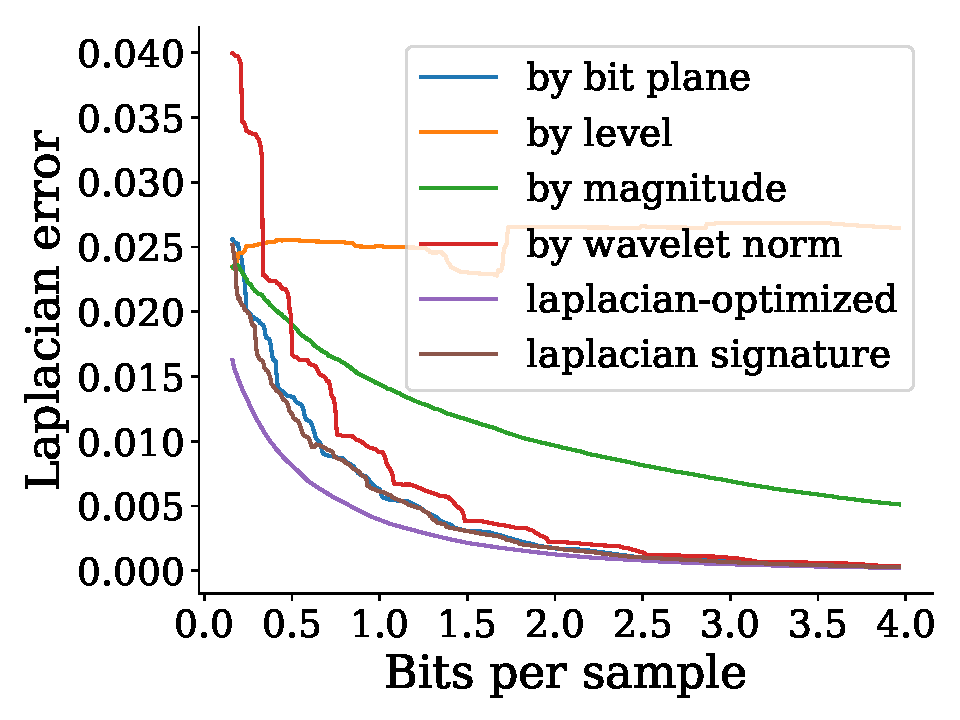
\includegraphics[width=0.24\linewidth]{laplacian/laplacian-optimized-diffusivity}}
\subcaptionbox{\emph{turbulence}}
{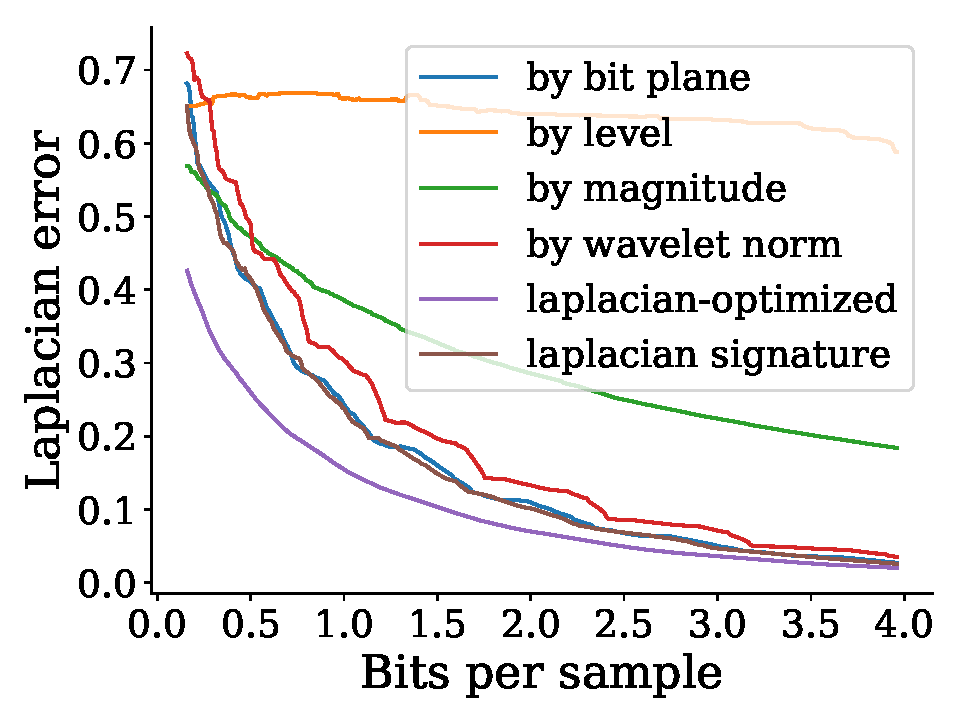
\includegraphics[width=0.24\linewidth]{laplacian/laplacian-optimized-turbulence}}
\subcaptionbox{\emph{pressure}}
{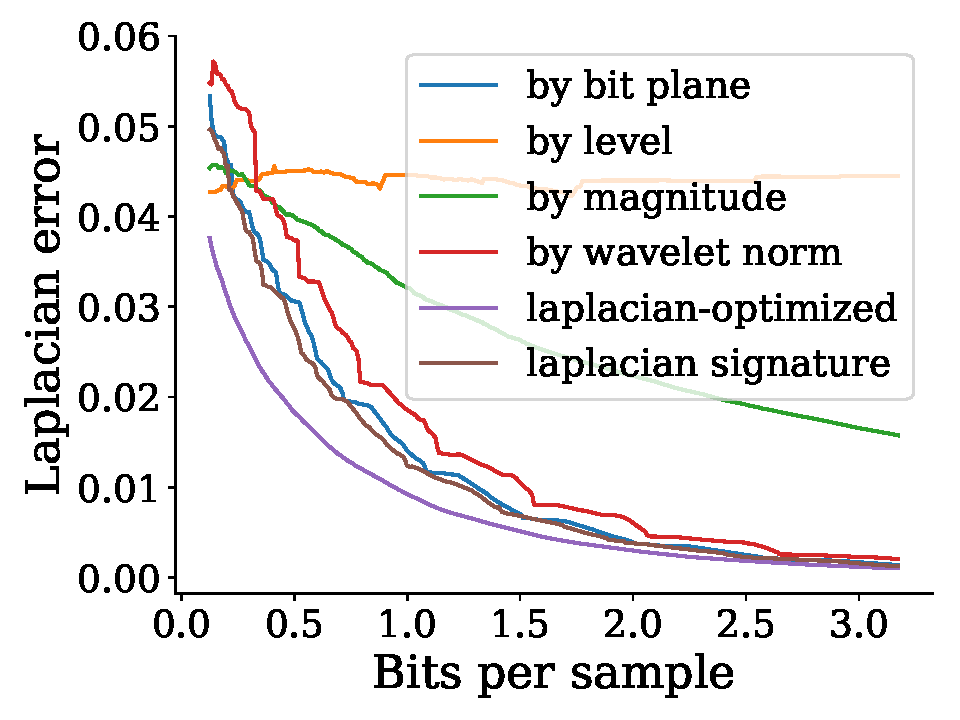
\includegraphics[width=0.24\linewidth]{laplacian/laplacian-optimized-pressure}}
\caption{Laplacian error comparison among streams, using the three-point \hb{or 5?}
stencil. The plots are truncated so as to better highlight differences without
discarding important information. In all cases, \emph{Laplacian}\pavol{finish}}
\label{fig:laplacian-error-comparison}
\vspace{1em}

\centering
\subcaptionbox{\emph{by level} (\slvl)}
{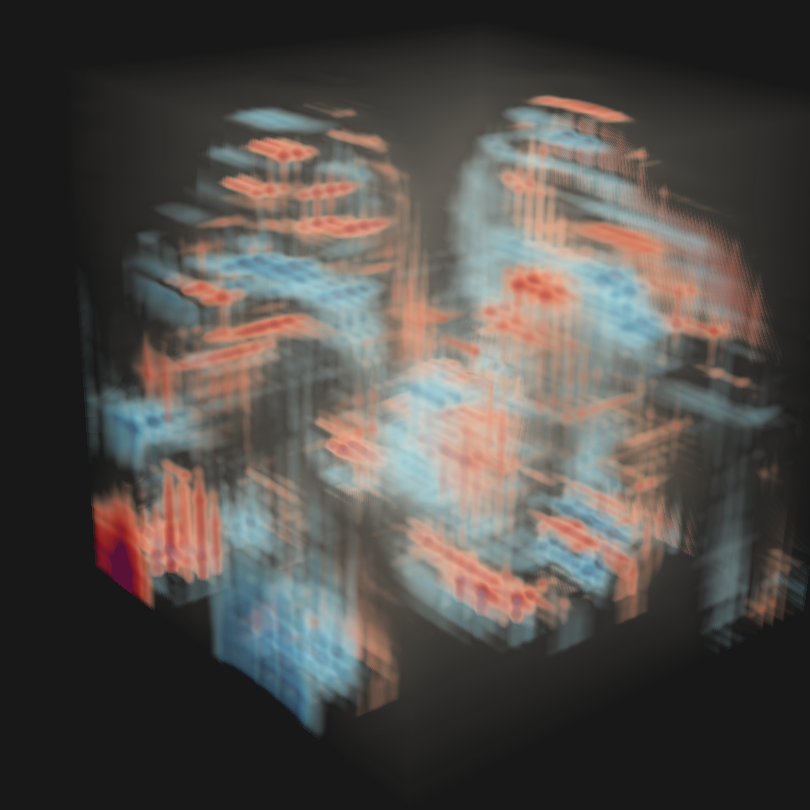
\includegraphics[width=0.16\linewidth]{laplacian/laplacian-pressure-level}}
\subcaptionbox{\emph{by bit plane} (\sbit)}
{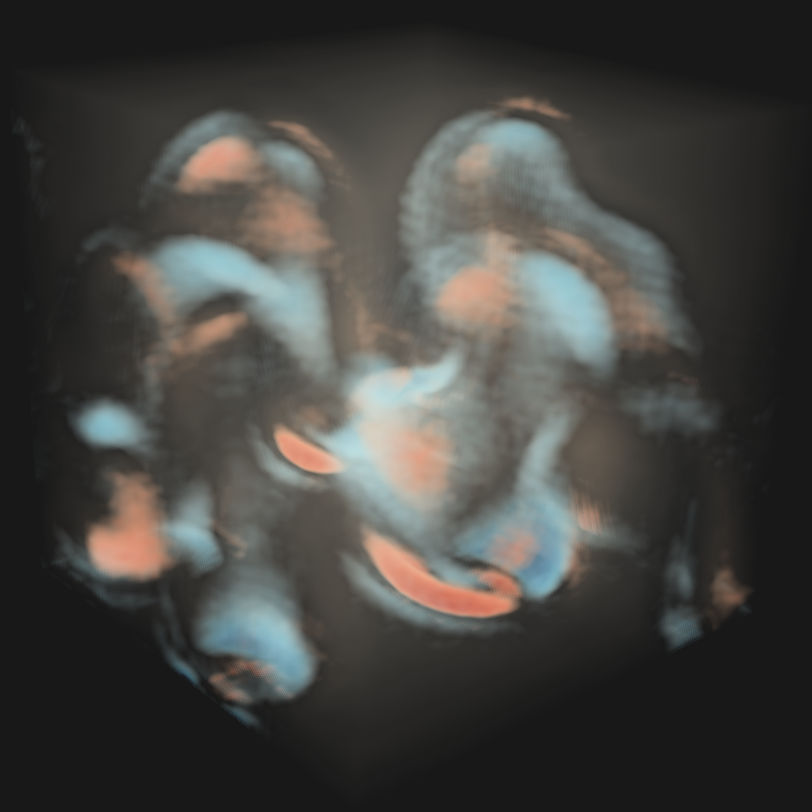
\includegraphics[width=0.16\linewidth]{laplacian/laplacian-pressure-bit-plane}}
\subcaptionbox{\emph{by wavelet norm} (\swav)}
{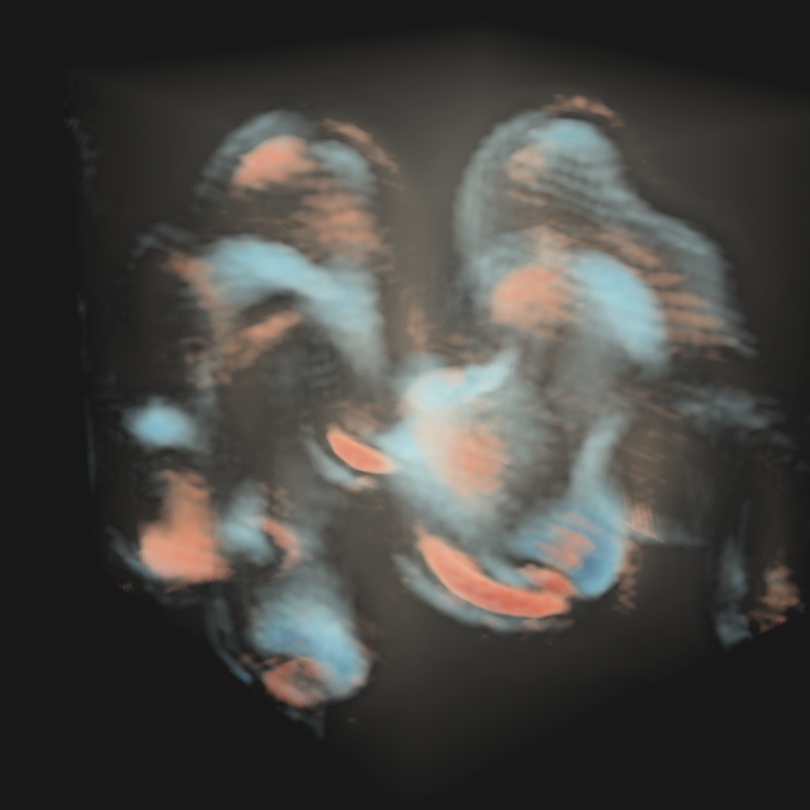
\includegraphics[width=0.16\linewidth]{laplacian/laplacian-pressure-wavelet-norm}}
\subcaptionbox{\emph{by magnitude} (\smag)}
{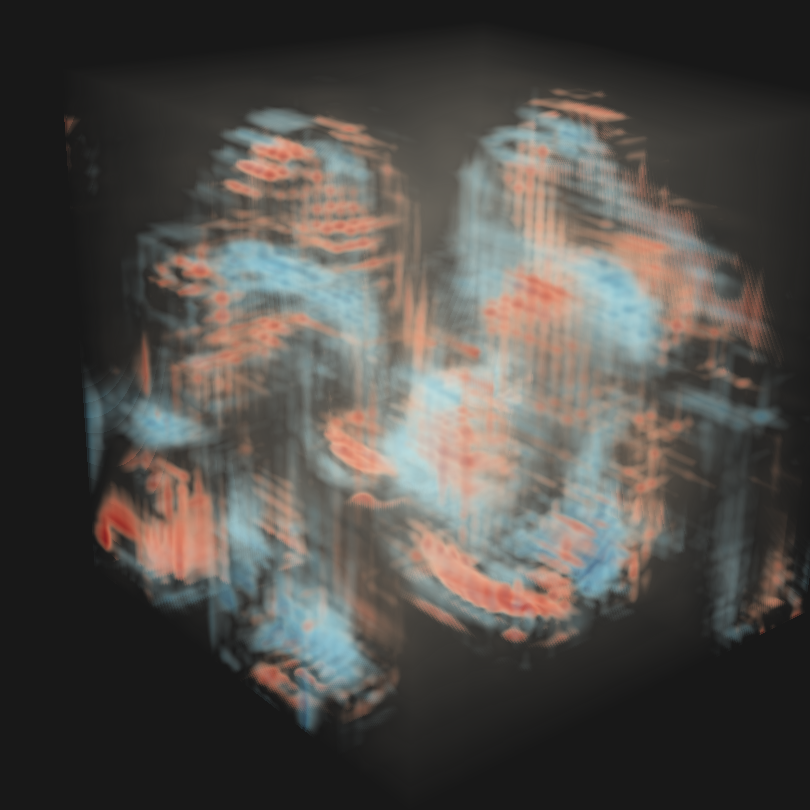
\includegraphics[width=0.16\linewidth]{laplacian/laplacian-pressure-magnitude}}
\subcaptionbox{\emph{by signature} (\slsg)}
{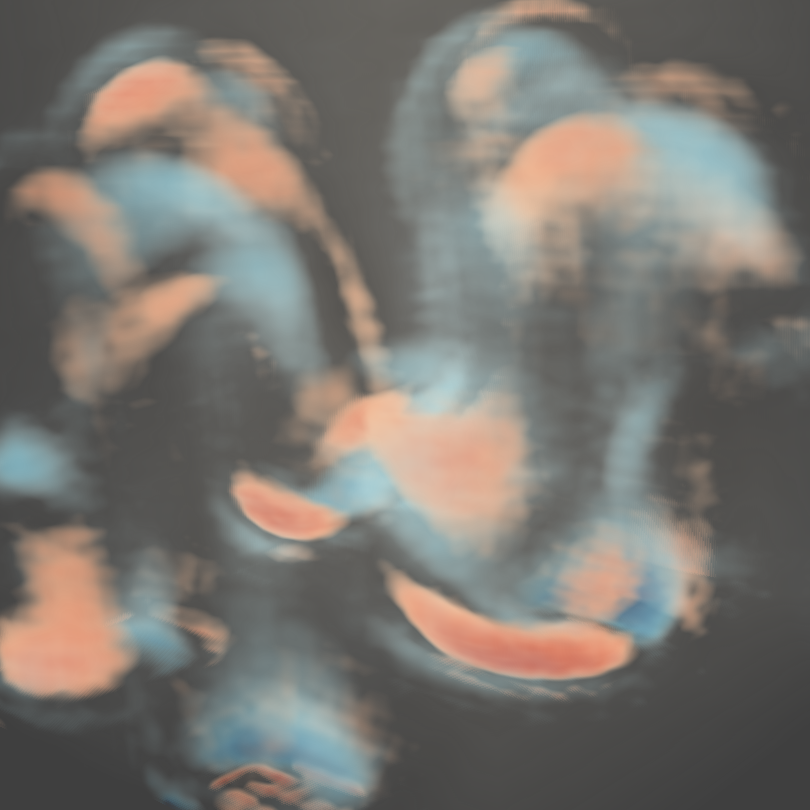
\includegraphics[width=0.16\linewidth]{laplacian/laplacian-pressure-signature}}
\subcaptionbox{\emph{ground truth}}
{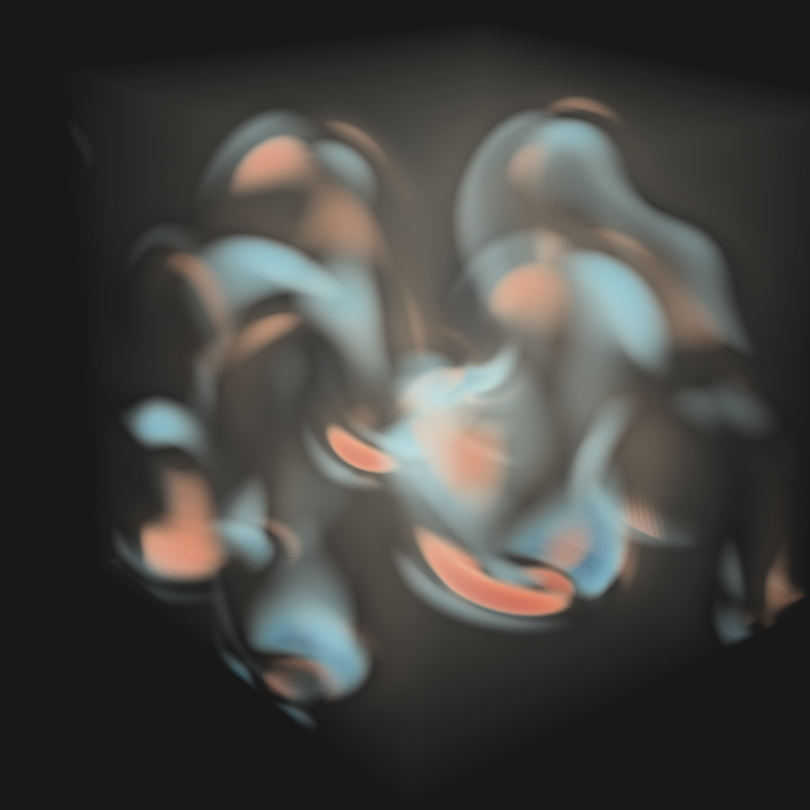
\includegraphics[width=0.16\linewidth]{laplacian/laplacian-pressure-groundtruth}}
\caption{Renderings of recontructed Laplacian fields for a $64^3$ region in
\emph{pressure}, at 0.9 bps.  In terms of image quality, $\slsg > \sbit > \swav
> \smag > \slvl$.} \label{fig:laplacian-renderings}
\end{figure*}

The Laplace operator is a second-order differential operator, defined as the divergence of the
gradient field. It can be computed by summing second partial derivatives in all dimensions, e.g., in
3D: $\Delta
f=\frac{{\partial}^2}{\partial{x^2}}f+\frac{{\partial}^2}{\partial{y^2}}f+\frac{{\partial}^2}{\partial{y^2}}f$.
To compute the Laplacian, we use the five-point finite difference to approximate the second
derivative in each dimension: $\frac{{\partial}^2}{\partial{x^2}}f(x,y,z) \approx
-\frac{1}{12}f(x-2,y,z)+\frac{4}{3}f(x-1,y,z)+\frac{-5}{2}f(x,y,z)+\frac{4}{3}f(x+1,y,z)-\frac{1}{12}f(x+2,y,z)$.
To compare two Laplacian fields, we use the root-mean-square error, i.e., $\err(\Delta
\tilde{f},\Delta f)=\text{RMSE}(\Delta \tilde{f},\Delta f)$. As usual, we use~\Cref{alg:greedy} to
compute a \emph{Laplacian-optimized} stream, \slop, which minimizes $\err$, and an \slsg stream from
its signature.~\Cref{fig:laplacian-error-comparison} plots the error curves for all relevant
streams. The plots here largely follow the one in~\Cref{fig:gradient-error-comparison}, in terms of
relative performance among the streams, with one minor discrepancy. \sbit consistently underperforms
\slsg by a small margin, and produces ``bumpier'' error curves (\todo{explain?}). In
\Cref{fig:laplacian-renderings}, we render the reconstructed Laplacian fields for the
\emph{pressure} field at 0.9 bps, which shows how differences in Laplacian among the streams
translate to visual differences.
